% Created 2014-02-27 Thu 12:38
\documentclass[11pt]{article}
\usepackage[utf8]{inputenc}
\usepackage[T1]{fontenc}
\usepackage{fixltx2e}
\usepackage{graphicx}
\usepackage{longtable}
\usepackage{float}
\usepackage{wrapfig}
\usepackage{soul}
\usepackage{textcomp}
\usepackage{marvosym}
\usepackage{wasysym}
\usepackage{latexsym}
\usepackage{amssymb}
\usepackage{hyperref}
\tolerance=1000
\usepackage[margin=0.75in]{geometry}
\providecommand{\alert}[1]{\textbf{#1}}

\title{Master Class Diagram}
\author{Ian Westrope, Keith Drew}
\date{2014-02-27 Thur}
\hypersetup{
  pdfkeywords={},
  pdfsubject={},
  pdfcreator={Emacs Org-mode version 7.9.3f}}

\begin{document}

\maketitle


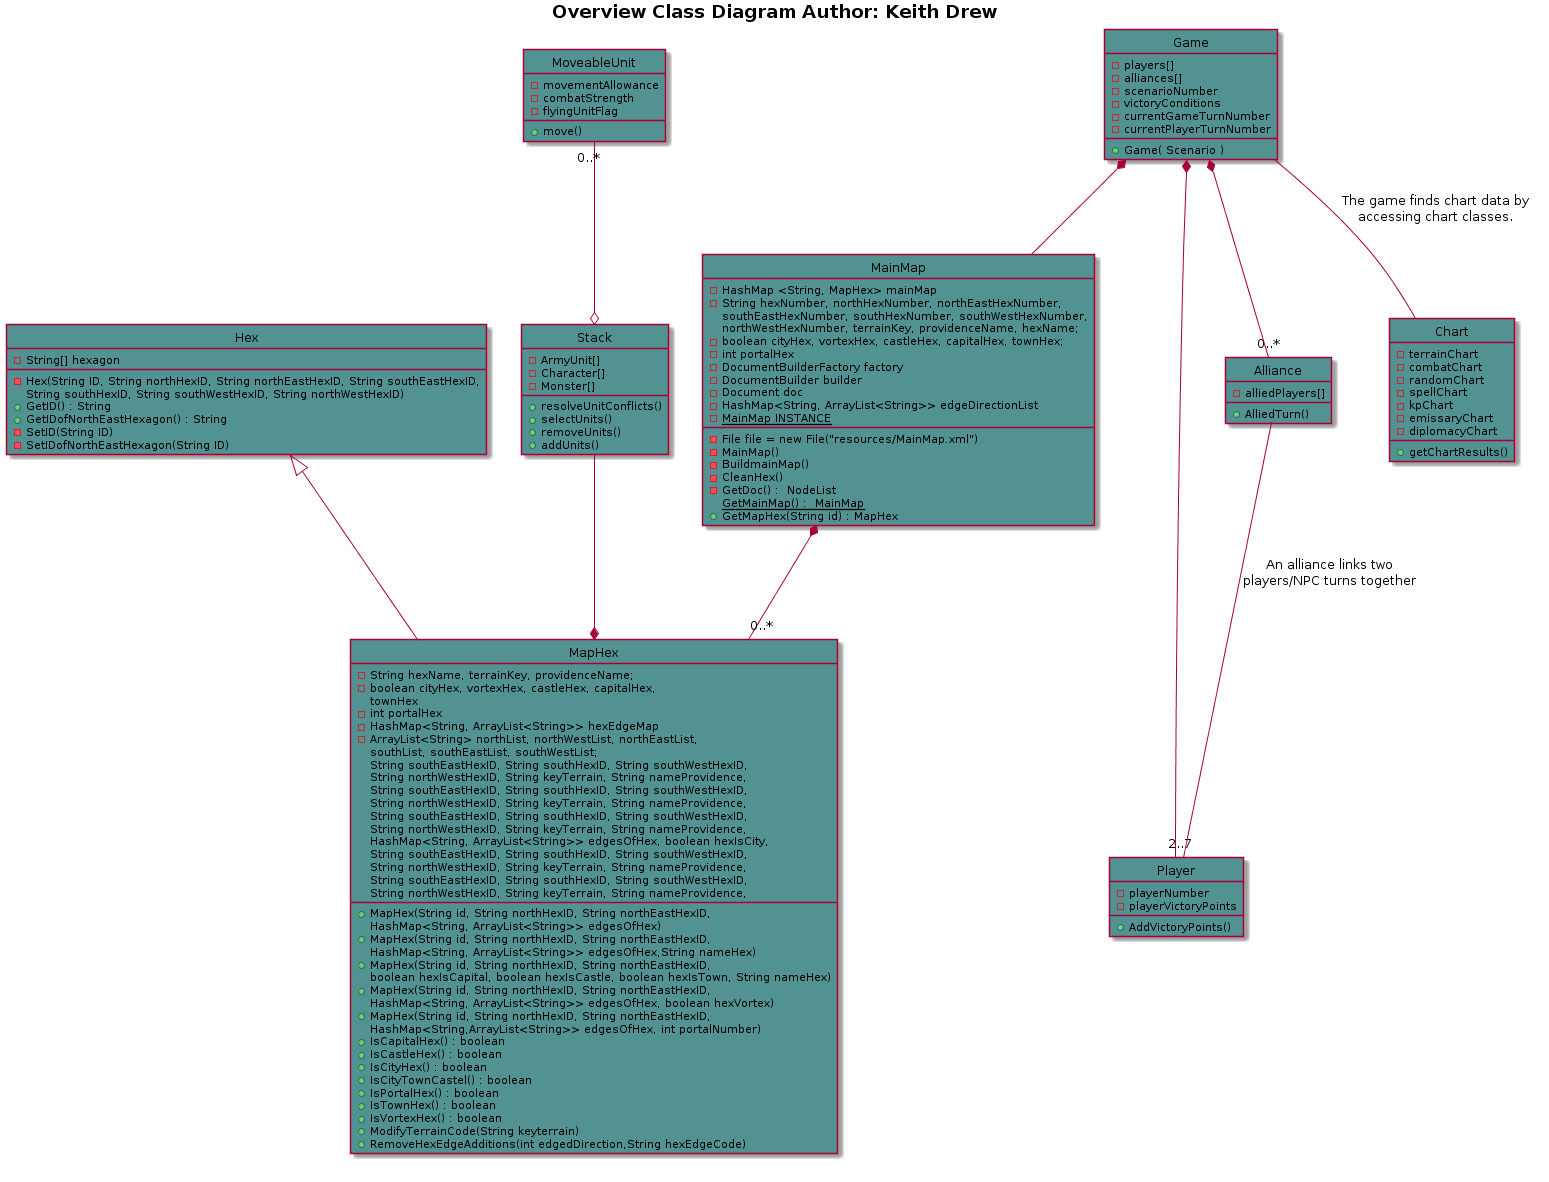
\includegraphics[width=\linewidth]{overview.png}
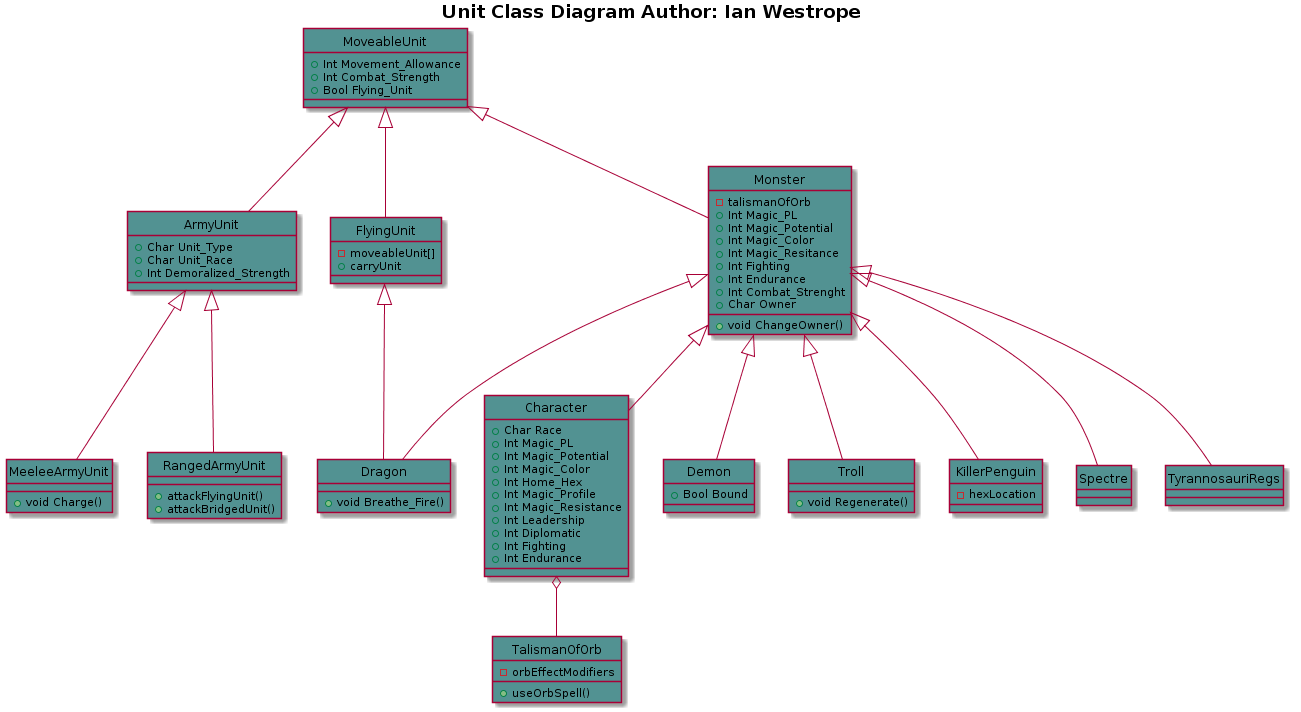
\includegraphics[width=\linewidth]{units.png}
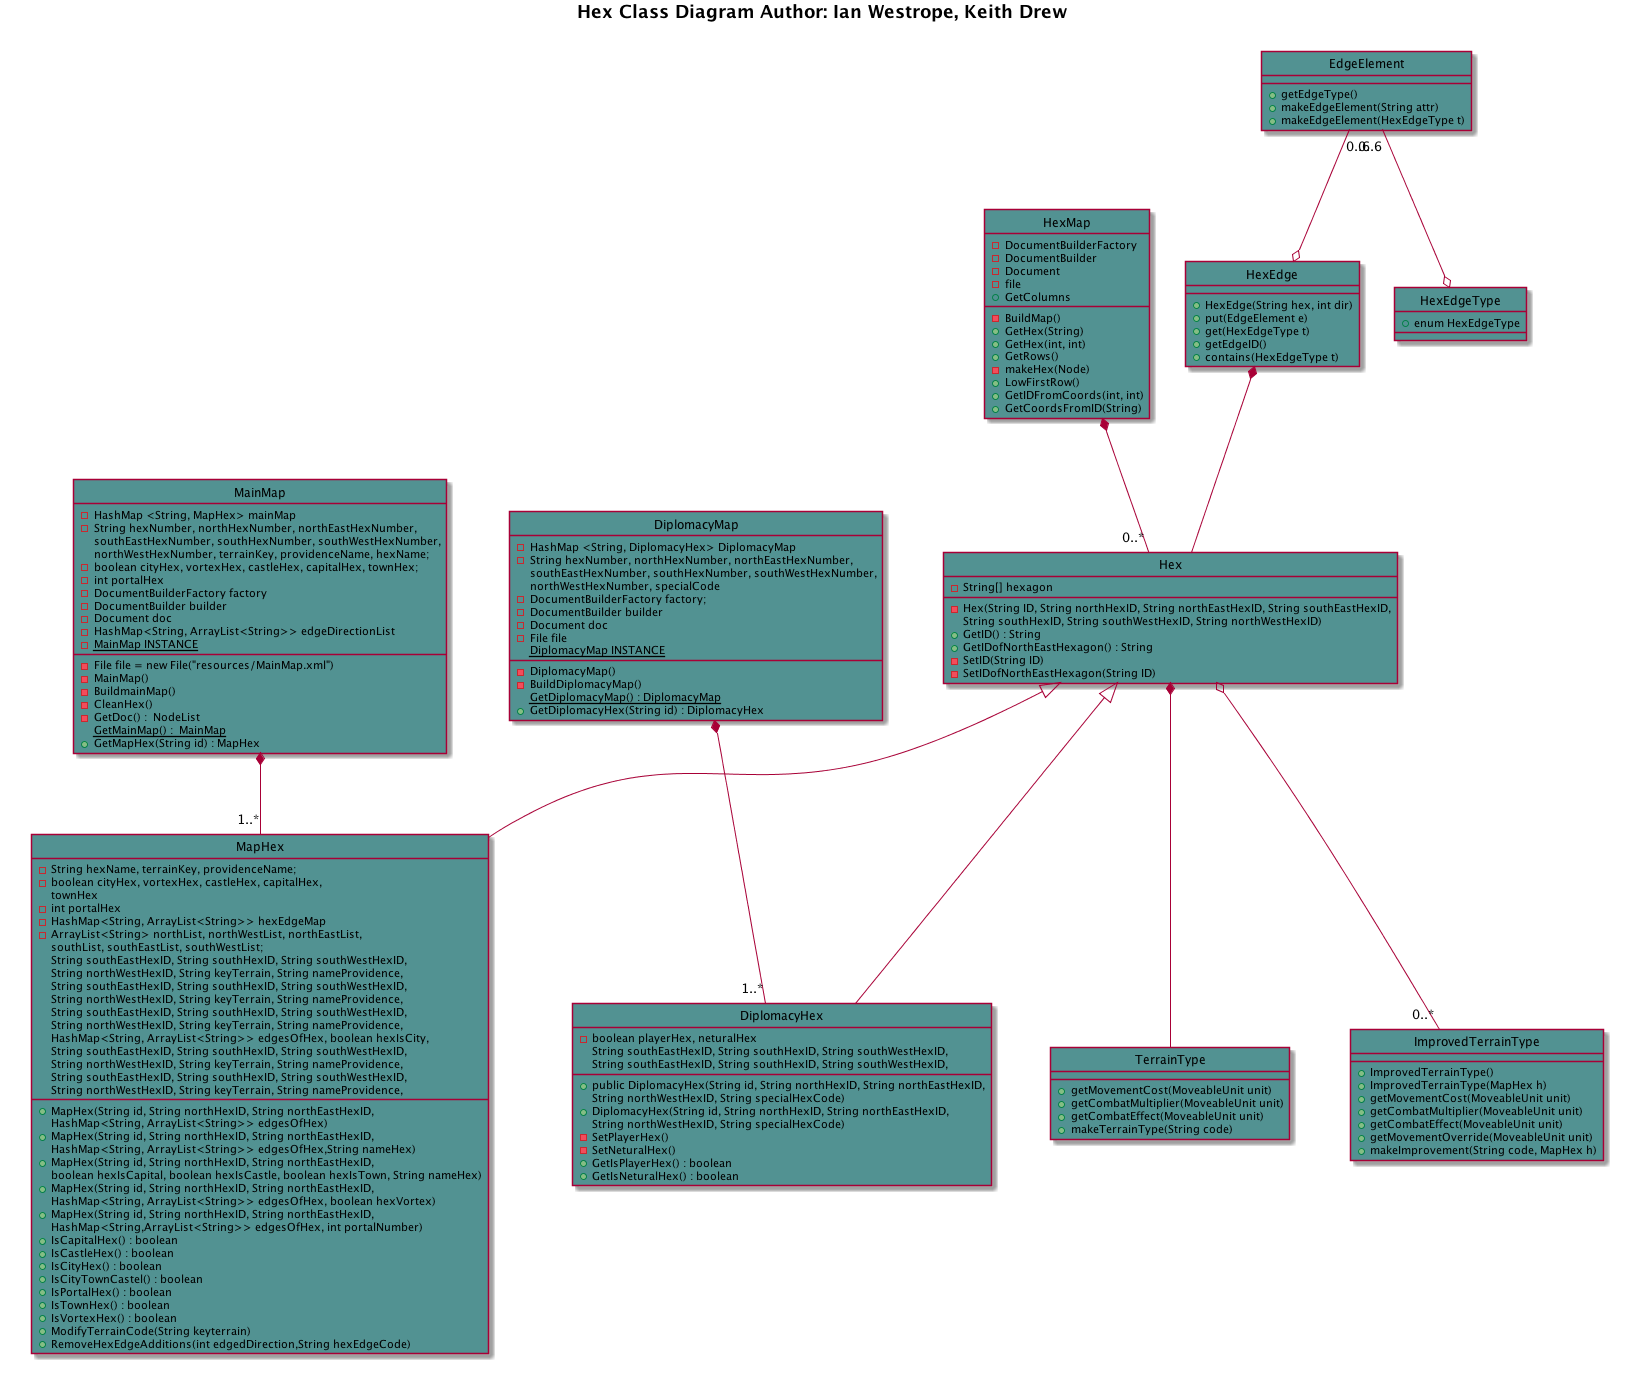
\includegraphics[width=\linewidth]{hex.png}
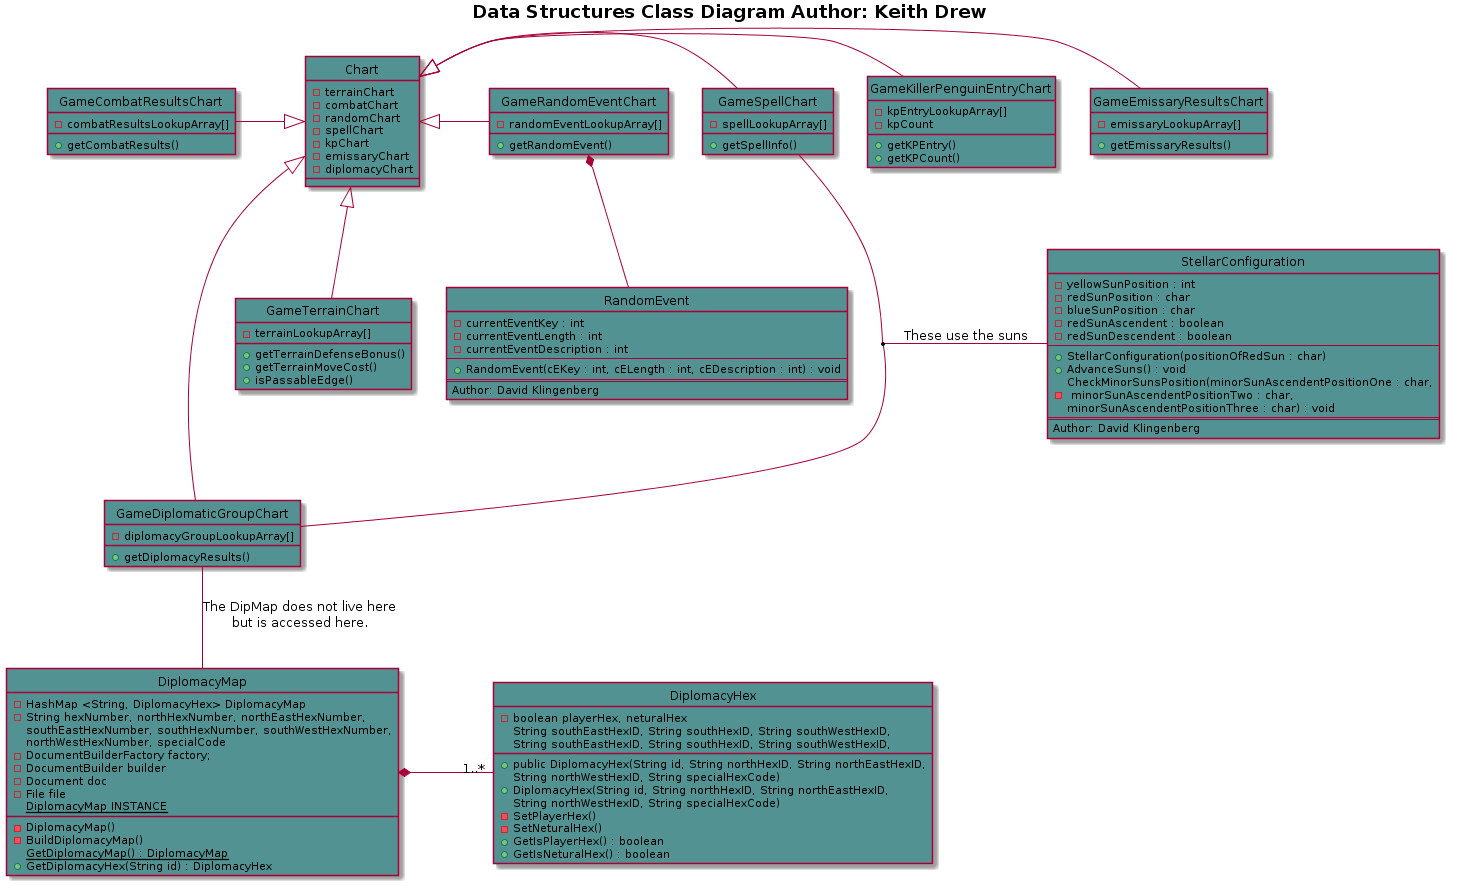
\includegraphics[width=\linewidth]{dataDiagram.png}


\section{Class Dictionary}
\label{sec-1}

\begin{description}
\item[Game:] An instance of the game, Swords and Sorcery
\item[Board:] The Board class is an aggregate class, made up of Provinces.
\item[Player:] An programming construct that represents a player at the ``board''. This includes factions, victory points, etc.
\item[Alliance:] The Alliance class is a that links two Players or NPCs together for a turn.
\item[Province:] The Province class is an aggregate class, made up of Hexes. It represents the different provinces found on the game map.
\item[Hex:] The Hex class is an aggregate class, made up of a Stack class. It represents the individual hexes found on the game map.
\item[Stack:] The Stack class is an aggregate class, made up of zero or more MoveableUnits.
\item[Moveable Unit:] MoveableUnit is the superclass for any object that can move in S\&S.
\item[Army Unit:] Simple units used for combat, limited to 2 per Stack object.
\item[Melee Army Unit:] Meellee Army Unit inherits from Army Unit. Meelee Army Unit represents both horsed and foot units from the game.
\item[Ranged Army Unit:] Ranged Army Unit inherits from Army Unit. Ranged Army Unit represents the units with bows from the game.
\item[Monster:] The Monster class inherits from MoveableUnit. It represents the monster units from the game.
\item[Character:] Character inherits from Monster and is also an aggregate class possibly made of TalismanOfOrb.
\item[Caster Character:] The class of characters that can use magic. This class includes methods for actually casting a given spell, made through a call to the appropriate data structure class.
\item[Fighter Character:] The class of characters that cannot use magic.
\item[Talisman Of Orb:] The class of magical items. This are held by certain characters and include methods that apply stat bonuses and methods that invoke certain spells.
\item[Scenario:] A premade instance of a game. The scenario both initializes a game and dictates any win conditions, number of players, and other meta-details about the game.
\item[DataController:] The class that holds all data chart classes. Through this class all data charts should be accessed.
\item[Game Combat Results Chart:] This chart class holds the data indicating combat results, as well as necessary methods that are intuitive to hold here.
\item[Game Terrain Chart:] This chart class holds necessary data and methods for determining terrain effects for defense bonuses and movement costs. This class also contains methods for altering hex types.
\item[Game Random Event Chart:] This chart class holds methods and data for determining random events for each game turn. The class includes methods to apply random event effects where needed.
\item[Game Spell Chart:] This chart class contains spell descriptions, spell casting charts, and the methods that are used to cast each spell. Casting a spell involves asking this class to execute a method.
\item[Game Killer Penguin Entry Chart:] This chart class determines how many (if any) Killer Penguins enter the field in given circumstances, and includes methods for adding the KPs to the field of play.
\item[Game Emissary Results Chart:] This chart includes the methods and data necessary to determine the results of an emissary's attempt to conduct diplomacy.
\item[Game Diplomatic Group Chart:] This chart class helps determine bonuses for diplomacy rolls, in conjunction with the emissary results table. It includes methods for returning the appropriate bonuses.
\end{description}

\end{document}
